
To help understand the requirements for an improvement in overall performance, models were constructed to estimate the amount of time spent fetching and decoding information.
Two models were constructed, an analytical model that did not consider processor level parallelism and a simulation-based model that considered certain processor level parallelism.
Both models are based on the sparse matrix-vector product, but, due to the similarity of the data access for the symmetric Gauss-Seidel step, should provide an estimate on both kernels.
Additionally, the models only provide estimates for rows with 27 elements, because there are \(O(n^3)\) of those rows and only \(O(n^2)\) of other rows where the matrix has \(O(n^3)\) rows.
Finally, the models assume that the compression does not reduce the rate of convergence.
The models were analyzed using the memory access latencies of the head node of the testing cluster.
These latencies are shown in Table~\ref{tab:models-baseLatencies}.
\begin{table}
	\centering
	\begin{tabular}{cc}
		L1 Cache Latency & 4-5 cycles \\
		L2 Cache Latency & 12 cycles \\
		L3 Cache Latency & 38 cycles \\
		Main Memory Latency & 38 cycles + 58 ns \\
		Clock Rate & 2.2GHz \\
	\end{tabular}
	\caption{Estimate cluster performance~\cite{7cpu:-:Bradwell}.}
	\label{tab:models-baseLatencies}
\end{table} %
The models were primarily used to find the minimum compression performance to outperform the baseline implementation.
The following variables represent the relevant compression characteristics in this section
\begin{align*}
	\mathrm{vectDecode} &= \text{time to decode one vector value} \\
	\mathrm{vectEncode}  &= \text{time to encode one vector value} \\
	\mathrm{vectBytes} &= \text{the number of bytes per vector value} \\
	\mathrm{matIndDecode} &= \text{time to decode one matrix index} \\
	\mathrm{matIndBytes} &= \text{the number of bytes per matrix index} \\
	\mathrm{matValDecode} &= \text{time to decode one matrix value} \\
	\mathrm{matValBytes} &= \text{the number of bytes per matrix value}
\end{align*}

Both models indicate that vector decoding must be incredibly efficient to see overall performance improvement, while matrix decoding can be less efficient.
This implies matrix compression has greater potential for overall performance improvement.
However, both models make significant assumptions and simplifications that limit the accuracy of these results.
Additionally, the models provide slightly different results.
For example, the analytical model indicates vector encoding time is negligible while the simulation model puts vector encoding time half the factor of vector decoding.

\subsection{Analytical Model}

The analytical model is a set of equations that computes the amount of time spent serially fetching and decoding the information.
This model is implemented using the following system of equations
\begin{align*}
	& 27\cdot \mathrm{vectDecode}+\mathrm{vectEncode} + 18\cdot \mathrm{L1Time} \\
	+ & \left(\frac{64-\mathrm{vectBytes}}{64}\cdot 9\cdot \mathrm{L1Time}+\frac{\mathrm{vectBytes}}{64}\cdot \left(6\cdot \mathrm{L2Time}+3\cdot \mathrm{RAMTime}\right)\right) \\
	+ & 27\cdot\mathrm{matIndDecode} \\
	+ & 27\cdot\left(\frac{\mathrm{matIndBytes}}{64}\cdot\mathrm{RAMTime} + \frac{64-\mathrm{matIndBytes}}{64}\cdot\mathrm{L1Time}\right) \\
	+ & 27\cdot\mathrm{matValDecode} \\
	+ & 27\cdot\left(\frac{\mathrm{matValBytes}}{64}\cdot\mathrm{RAMTime}+\frac{64-\mathrm{matValBytes}}{64}\cdot\mathrm{L1Time}\right)
\end{align*}
where
\begin{align*}
	\mathrm{L1Time} &= \text{the access latency for L1 cache} \\
	\mathrm{L2Time} &= \text{the access latency for L2 cache} \\
	\mathrm{RAMTime} &= \text{the access latency for main memory.} \\
\end{align*}
This model utilizes a few facts and assumptions.
Firstly, the number of bytes per value divided by 64 provides the percent of values that will require fetching a cache line from main memory or higher caches, while 1 minus this value is the percent of values that will be able to only need to access L1 cache.
Secondly, due to the matrix sparsity pattern, two thirds of vector readers will always be in L1 cache and, assuming there are \(96^3\) rows per process, two thirds of the remaining values will be in L2 cache.
The model was only studied using the performance characteristics shown in Table~\ref{tab:models-baseLatencies}.
This model was used to create approximate bounds that need to be met to outperform the baseline implementation.
The model can be simplified by letting
\begin{align*}
\mathrm{decode} =& \mathrm{vectDecode} + \mathrm{matValDecode} + \mathrm{matIndDecode} \\
\mathrm{matBytes} =& \mathrm{matValBytes} + \mathrm{matIndBytes}.
\end{align*}
Then, the performance bounds are, approximately,
\begin{align*}
\mathrm{vectEncode} <& 878.513 \\
\mathrm{decode} <& 32.5375 - 0.037037\cdot\mathrm{vectEncode} \\
\mathrm{matBytes} <& 12.9664 - 0.398506\cdot\mathrm{decode}- 0.0147595\cdot\mathrm{vectEncode}\\
\mathrm{vectBytes} <& 107.34  - 3.29897\cdot\mathrm{decode} - 0.122184\cdot\mathrm{vectEncode} \\
	&- 8.27835\cdot\mathrm{matBytes}\\
\end{align*}
where all encode and decode times are in clocks.
Note that the upper bound on the number of bytes per vector value is reduced by 3.29897 per 1 clock increase in decode time.
This indicates that only highly effective compression techniques will be effective for vector values.
Matrix compression on the other hand, appears to be able to achieve a performance improvement with a slower decompression than required by the vector values.

\subsection{Simulation Based Model}
The parallel model attempts to estimate the performance required to outperform the baseline implementation while considering processor level parallelism.
Figure~\ref{fig:models-dataDeps} shows the dependencies used by each model.
\begin{figure}
	
	\ifdraft{}{
		\begin{subfigure}[t]{0.34\textwidth}
			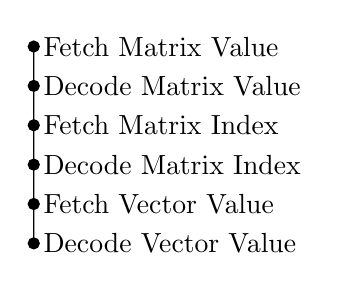
\begin{tikzpicture}
				\filldraw
					(0,2.5) circle (2pt) node[right] {Fetch Matrix Value} --
					(0,2.0) circle (2pt) node[right] {Decode Matrix Value} --
					(0,1.5) circle (2pt) node[right] {Fetch Matrix Index} --
					(0,1.0) circle (2pt) node[right] {Decode Matrix Index} --
					(0,0.5) circle (2pt) node[right] {Fetch Vector Value} --
					(0,0.0) circle (2pt) node[right] {Decode Vector Value};
			\end{tikzpicture}
			\caption{Serial Model.}
		\end{subfigure}
		\begin{subfigure}[t]{0.65\textwidth}
			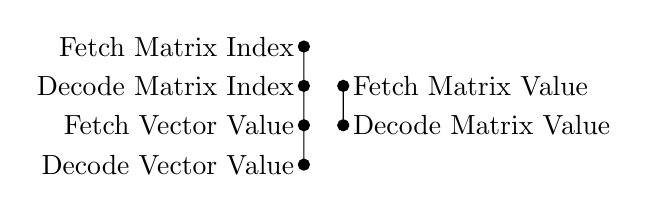
\begin{tikzpicture}
				\filldraw
					(0,2.0) circle (2pt) node[left] {Fetch Matrix Index} --
					(0,1.5) circle (2pt) node[left] {Decode Matrix Index} --
					(0,1.0) circle (2pt) node[left] {Fetch Vector Value} --
					(0,0.5) circle (2pt) node[left] {Decode Vector Value};
				\filldraw
					(0.5,1.5) circle (2pt) node[right] {Fetch Matrix Value} --
					(0.5,1.0) circle (2pt) node[right] {Decode Matrix Value};
			\end{tikzpicture}
			\caption{Parallel Model.}
		\end{subfigure}
	}
	
	\caption[Data dependency graphs for performance models.]{Comparison of the data dependency graphs used by each model, where lower nodes are dependent on higher nodes.}
	\label{fig:models-dataDeps}
\end{figure} %
Note that this model assumes that the compiler and processor can fully parallelize any operations without data dependencies, while, the instructions must be at least read serially~\cite{Hennessy:1990:ComputerArchitecture}.
Additionally, the model assumes that the bytes of each compressed value is constant, which is not true for most matrix compression and for some vector compression.
Also, the model was not used to analyze compressing multiple data structures simultaneously due to the difficulty of analyzing the resulting seven-dimension region.
Lastly, the model was used with integral values for the bytes, decode times and encode times.
The model then takes the same compression properties as the first model and computes the time to fetch and decode the values and encode the result value over 10 matrix rows with 27 entries per row.
Appendix~\ref{app:decode-model-source} contains source code for this model.

The bounds on outperforming the baseline implementation were hard to determine for the simulation model due to the nature of the model as a sum of maximizations.
However, some boundaries were computed.
Table~\ref{tab:models-singleComp} shows the restrictions when compressing only a single data structure.
\begin{table}
	\begin{tabular}{r|S|S|c}
      & {Matrix Index}  & {Matrix Value} & {Vector}\\
	{Bytes} & {Decode}        & {Decode}       & Encode and Decode \\
	\hline
	1 & 66 & 41 & \(4.75\geq 1.75\cdot\mathrm{decode}+\mathrm{encode}\)\\
	2 & 51 & 14 &\(4.75\geq 1.75\cdot\mathrm{decode}+\mathrm{encode}\)\\
	3 & 66 & 40 &\(2\geq 2\cdot\mathrm{decode}+\mathrm{encode}\)\\
	4 & 0 & 0 &\(0=\mathrm{decode}=\mathrm{encode}\) \\
	5 & {-} & 37 & \(4.75\geq 1.75\cdot\mathrm{decode}+\mathrm{encode}\)\\
	6 & {-} & 9 & Not Possible\\
	7 & {-} & 35 & \(0=\mathrm{decode}=\mathrm{encode}\)\\
	8 & {-} & 0 & \(0=\mathrm{decode}=\mathrm{encode}\)
\end{tabular}

	\caption{Maximum Decode Times in Clocks for Single Structure Compression According to the Simulation Based Model.}
	\label{tab:models-singleComp}
\end{table} %
The matrix index and value columns contain the maximum time to decode a value, in clocks.
The vector column contains equations that restrict the decode and encode time, with values in clocks.
Note that the vector limits are not the only way to compute the restriction.
These compression bounds appear to be significantly related to the frequency at which multiple values are fetched from main memory simultaneously.
